\subsubsection{Pixel Formats}
\label{subsubsec:pixel_format}
% \todo[inline]{Citations, Document, that only 8bits are used? No.}
% (https://en.ids-imaging.com/tl_files/downloads/techtip/TechTip_18MP-color-sensor-as-mono_EN.pdf)

The Baumer industrial camera VCXU-13C uses the digital image sensor PYTHON1300 from ON Semiconductor and allows for the use of monochrome, raw and color pixel formats (see chapter \ref{sec:camera}).
The digital image sensor itself has 1280 $\times$ \SI{1024}{px} that acquire brightness with a bit depth of \SI{10}{bit}.
In order to capture color images, a color filter is applied to each individual pixel.
These red, green and blue (RGB or BGR) color filters only transmit light with a particular wavelength.
Due to the fact that the luminance perception of the human eye is most sensitive to green light, twice as many green filters are used as red and blue filters.
The color filters are arranged in a Bayer color matrix $B$, as shown in figure \ref{subfig:bayerrg} \cite{dcs}.

There are several modifications of the Bayer pattern that can be achieved by simply shifting the pixels around.
The pattern in figure \ref{subfig:bayergr} is achieved by shifting the initial pattern one pixel to the left, whereas the pattern in figure \ref{subfig:bayergb} is achieved by shifting the pattern one pixel up.

The different Bayer patterns are usually named after the color of the elements $B_{1,1}$, $B_{1,2}$, $B_{2,1}$ and $B_{2,2}$.
This results in the four possible patterns \texttt{RGGB}, \texttt{GRBG}, \texttt{GBRG} and \texttt{BGGR}.

However, there exist different naming conventions for the different Bayer patterns.
Baumer labels the Bayer patterns after the color of the elements $B_{1,1}$ and $B_{1,2}$, resulting in the name \texttt{BayerRG} for figure \ref{subfig:bayerrg}.
The Open Computer Vision Library (OpenCV) labels them after the elements $B_{2,2}$ and $B_{2,3}$, resulting in the name \texttt{BayerBG} for the same figure \ref{subfig:bayerrg} \cite{baumer_opencv}.

In order to create an RGB color image from the raw Bayer pattern image, a demosaicing (also ``debayering'') algorithm is necessary.
The Baumer industrial camera VCXU-13C is able to transform the raw sensor data into the respective RGB or BGR values in real time.
Another possibility is to do the required color space transformation with the OpenCV function \texttt{cv::cvtColor}.
Since OpenCV uses the BGR instead of the standard RGB color space, the required color space conversion code is \texttt{cv::COLOR\_BayerBG2BGR}.
This will convert the raw Bayer pattern image into a BGR image \cite{opencv_csc}.

\begin{figure}[ht]
  \centering
  \begin{subfigure}[b]{0.3\textwidth}
    \centering
    \includegraphics[scale=1]{bayerrg}
    \caption{\texttt{RGGB} (Baumer \texttt{BayerRG})}
    \label{subfig:bayerrg}
  \end{subfigure}
  \begin{subfigure}[b]{0.3\textwidth}
    \centering
    \includegraphics[scale=1]{bayergr}
    \caption{\texttt{GRBG} (Baumer \texttt{BayerGR})}
    \label{subfig:bayergr}
  \end{subfigure}
  \begin{subfigure}[b]{0.3\textwidth}
    \centering
    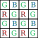
\includegraphics[scale=1]{bayergb}
    \caption{\texttt{GBRG} (Baumer \texttt{BayerGB})}
    \label{subfig:bayergb}
  \end{subfigure}
  \caption{Bayer color matrices $B$}
  \label{fig:bayer}
\end{figure}
